\section{Spannungsversorgung}\label{sec.spannungsversorgung}
In diesem Abschnitt soll auf die hardwareseitige Umsetzung der Spannungsversorgung für die Wetterstation eingegangen werden. Ziel ist der Entwurf einer Platine, auf der sämtliche Anforderungen umgesetzt werden.

\subsection{Anforderungen}\label{subsec.anforderungen}
Zunächst sollen in diesem Abschnitt die Anforderungen, die sich aus der Aufgabenstellung ableiten lassen, sowie solche, die sich aus den weiteren Überlegungen zur Umsetzung der Wetterstation ergeben.

\begin{itemize}

	\item Messung des Ladestroms
	\item Messung der Batteriespannung (Ladezustand)
	\item Messung des Stromverbrauchs der Wetterstation

\end{itemize}

Des Weiteren soll der Stromverbrauch der Wetterstation so niedrig wie möglich sein, um die Puffer-Batterie zu schonen und sonnenarme Phasen bzw. die Nacht ohne Stromausfall überbrücken zu können. Die verwendete Batterie hat eine Ladeschlussspannung von 12\,V. Da für den Mikrocontroller und die Sensoren allerdings Spannungspegel von 3,3\,V und 5\,V benötigt werden, müssen diese auf der Platine erzeugt werden.

Aus den mechanischen Anforderungen, dass Mikrocontroller, Platine und Sensoren möglichst in einem Gehäuse untergebracht werden sollen, ergibt sich, dass 
%Messaufgaben, Stromverbrauch, 3v3 5v
\subsection{Erzeugung benötigter Spannungen}\label{subsec.Spannungserzeugung}

\subsection{Spannungsabschaltung}\label{subsec.Spannungsabschaltung}

\subsection{Messung Strom/Spannung}\label{subsec.MessungStromSpannung}

\subsection{Beschaltung Sensoren}\label{subsec.BeschaltungSensoren}



%\begin{figure}[hbtp]
%  \centering
%  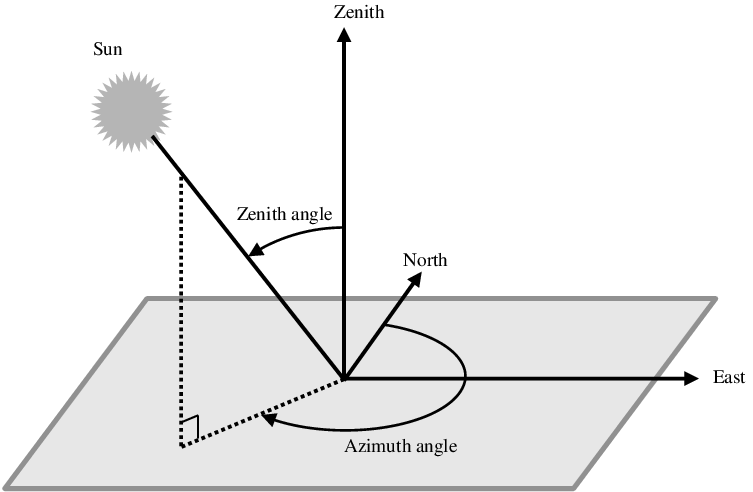
\includegraphics[width=\textwidth]{./img/Representation-of-azimuth-and-zenith-angles.png}
%  \caption{Beschreibung der Sonnenposition durch Zenith und Azimut~\cite{Nou2016}}\label{fig:zen_azi}
%\end{figure}